\documentclass{beamer}
\usetheme{default}
\setbeamertemplate{navigation symbols}{} % No navigation symbols
\usecolortheme[named=white]{structure} % White titles and such
\setbeamercolor{normal text}{fg=white} % White text
\setbeamercolor{background canvas}{bg=black} % Black background
% Comment this line for default bullet points (triangles)
\setbeamertemplate{itemize item}{\color{white}$\bullet$} 

\begin{document}

% {{{ Thoughts

% The Effects of Slavery and Colonialism on Contemporary African Politics

% Nathan Nunn on the effects of the West African slave trade
	% Not just West Africa, try to find some numbers on the East African
	% slave trade.

% Colonialism on the number of states, initial dead drop, only partial
% restoration in 60s -> our paper and paine, 
% BUT, lots of *polities* survived.
% Surprisingly light (institutional/administrative/manpower) imprint of
% colonialism. Strengthening the influence/prerogative/internal "power" of local
% rulers. (Why many were willing subjects). THIS has a big impact locally.
% Nationally, western *ideas* and the opening of the world is key, and in
% opposition to the development at the local level. Often excluding traditional
% leaders from power. Most/many regimes upon independence were led by the
% resistance to the colonial regime, of which traditional leaders were a key
% part.

% Ideas of democracy or at least modernization along western lines. Efforts to
% industrialize based on importing equipment, subsidizing urban areas (food and
% fuel) by exporting raw materials and agricultural products (infrastructure in
% place from colonialism). Effective way of taxing population at low political
% cost and with minimal administration involved. Also massive loans. Everything
% collapsed in the 80s and 90s when food prices collapsed.
% Industrialisation/development projects were in large part ill conceived and
% their proximity to the political process and systems of subsidies, made for a
% system rife with corruption. "Neo-colonialism" and IMF/World Bank austerity is
% not to blame. If anything IMF/World Bank should probably have had/demanded
% even more control. All of this has of course led to the familiar political
% legacy of (1) African states on the brink of bankruptcy, spending considerable
% part of their budget to service dept, (2) governments being a surprisingly
% large (corrupt, and inefficient) part of the (official) economy, (3) expensive
% subsidy systems that create black markets and smuggling across boundaries.

% }}}

\begin{frame}
\end{frame}

\setbeamercolor{background canvas}{bg=white}

\begin{frame}
	\begin{figure}
		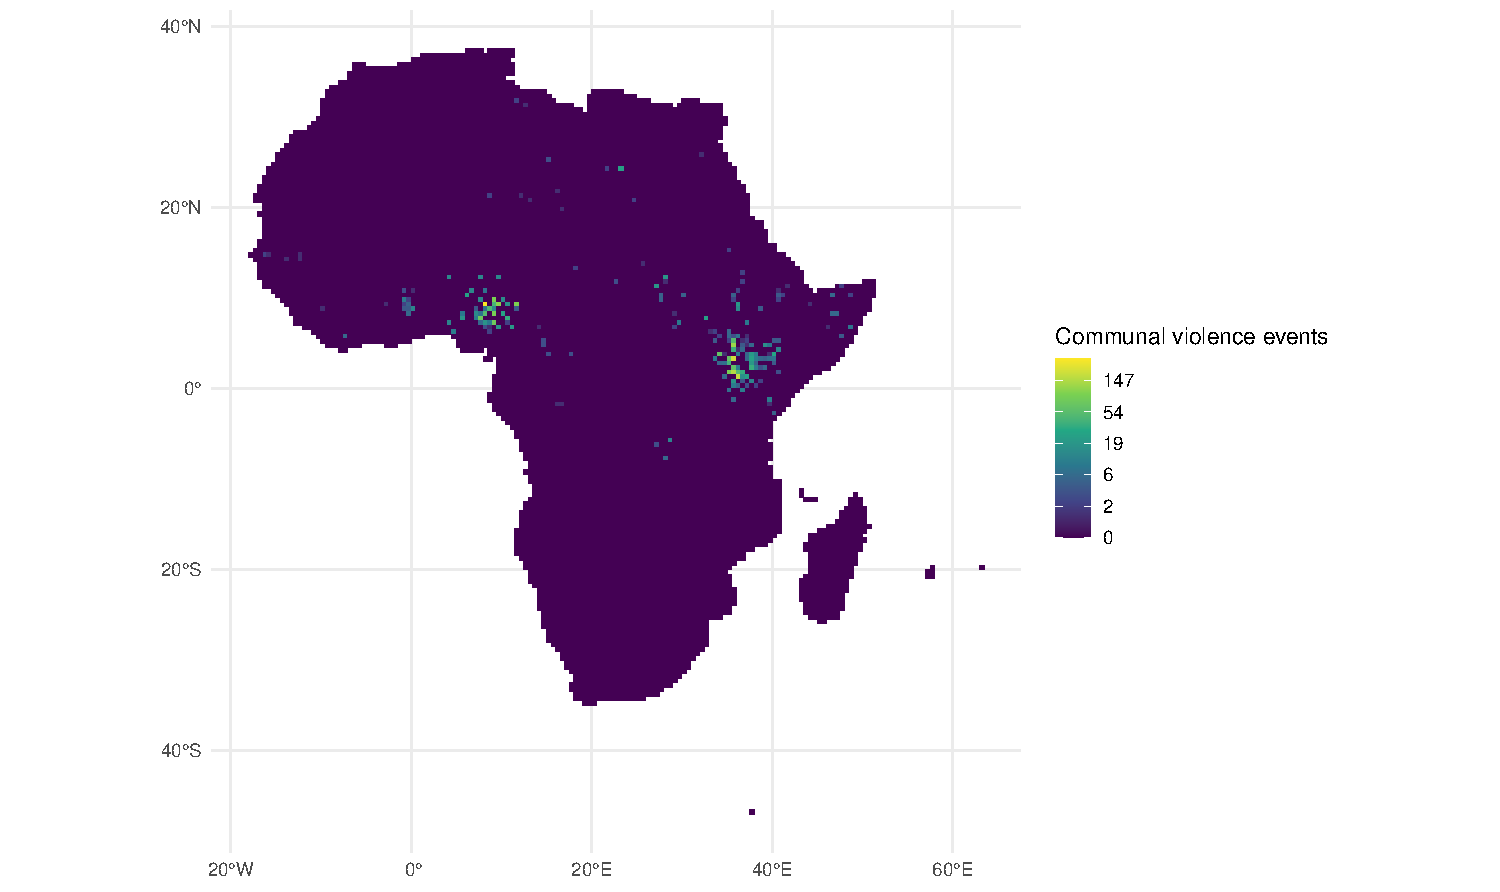
\includegraphics[width=\linewidth]{../R/Output/logOrg3.pdf}
	\end{figure}
\end{frame}

\setbeamercolor{background canvas}{bg=black}

\begin{frame}
\end{frame}

\begin{frame}
	\begin{figure}
		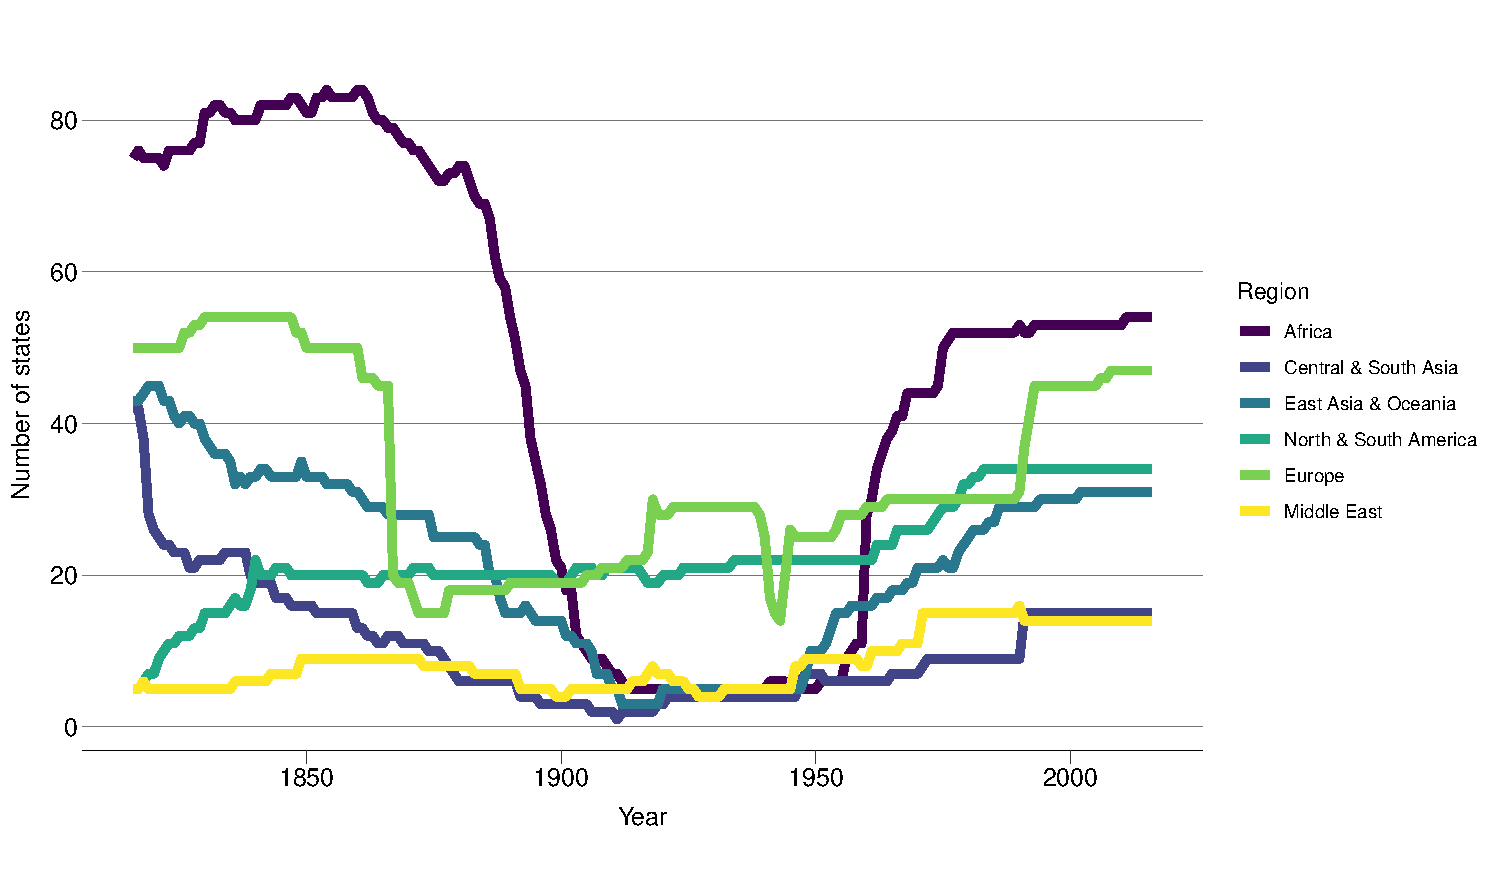
\includegraphics[width=\textwidth]{../R/Output/statesPerYear.pdf}
		\caption{The number of independent states per year.}
		\label{statesperyear}
	\end{figure}
\end{frame}

\setbeamercolor{background canvas}{bg=black}

\begin{frame}
\end{frame}

\setbeamercolor{background canvas}{bg=white}

\begin{frame}
	\begin{figure}
		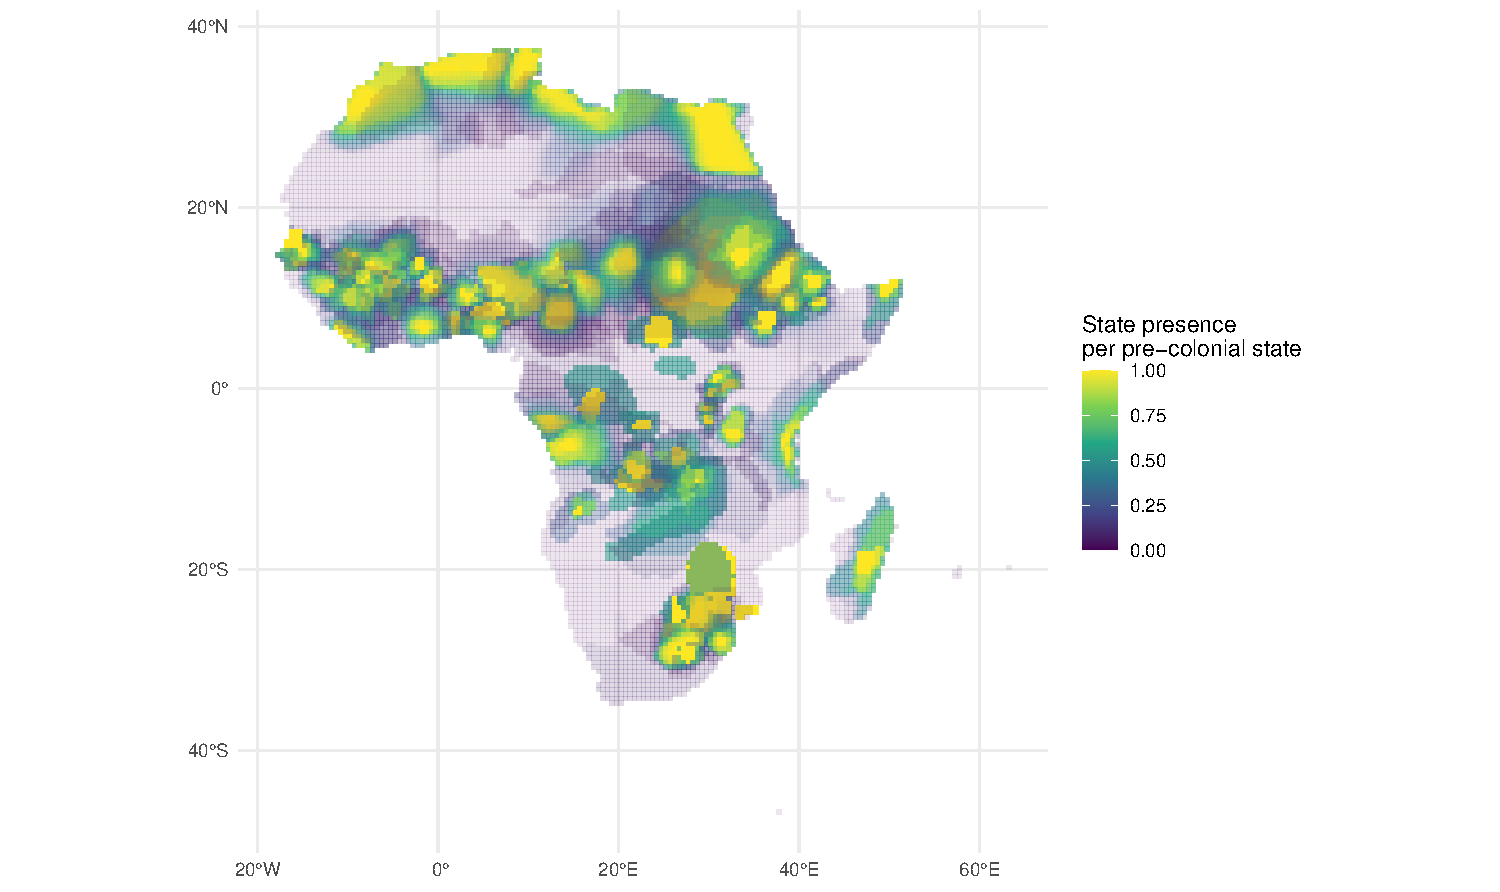
\includegraphics[width=\textwidth]{img/geo_isd_all.pdf}
		\caption{Pre-colonial state presence (normalized per pre-colonial state)}
	\end{figure}

\end{frame}

\setbeamercolor{background canvas}{bg=black}

\begin{frame}
\end{frame}

\setbeamercolor{background canvas}{bg=white}

\begin{frame}
	\begin{figure}
		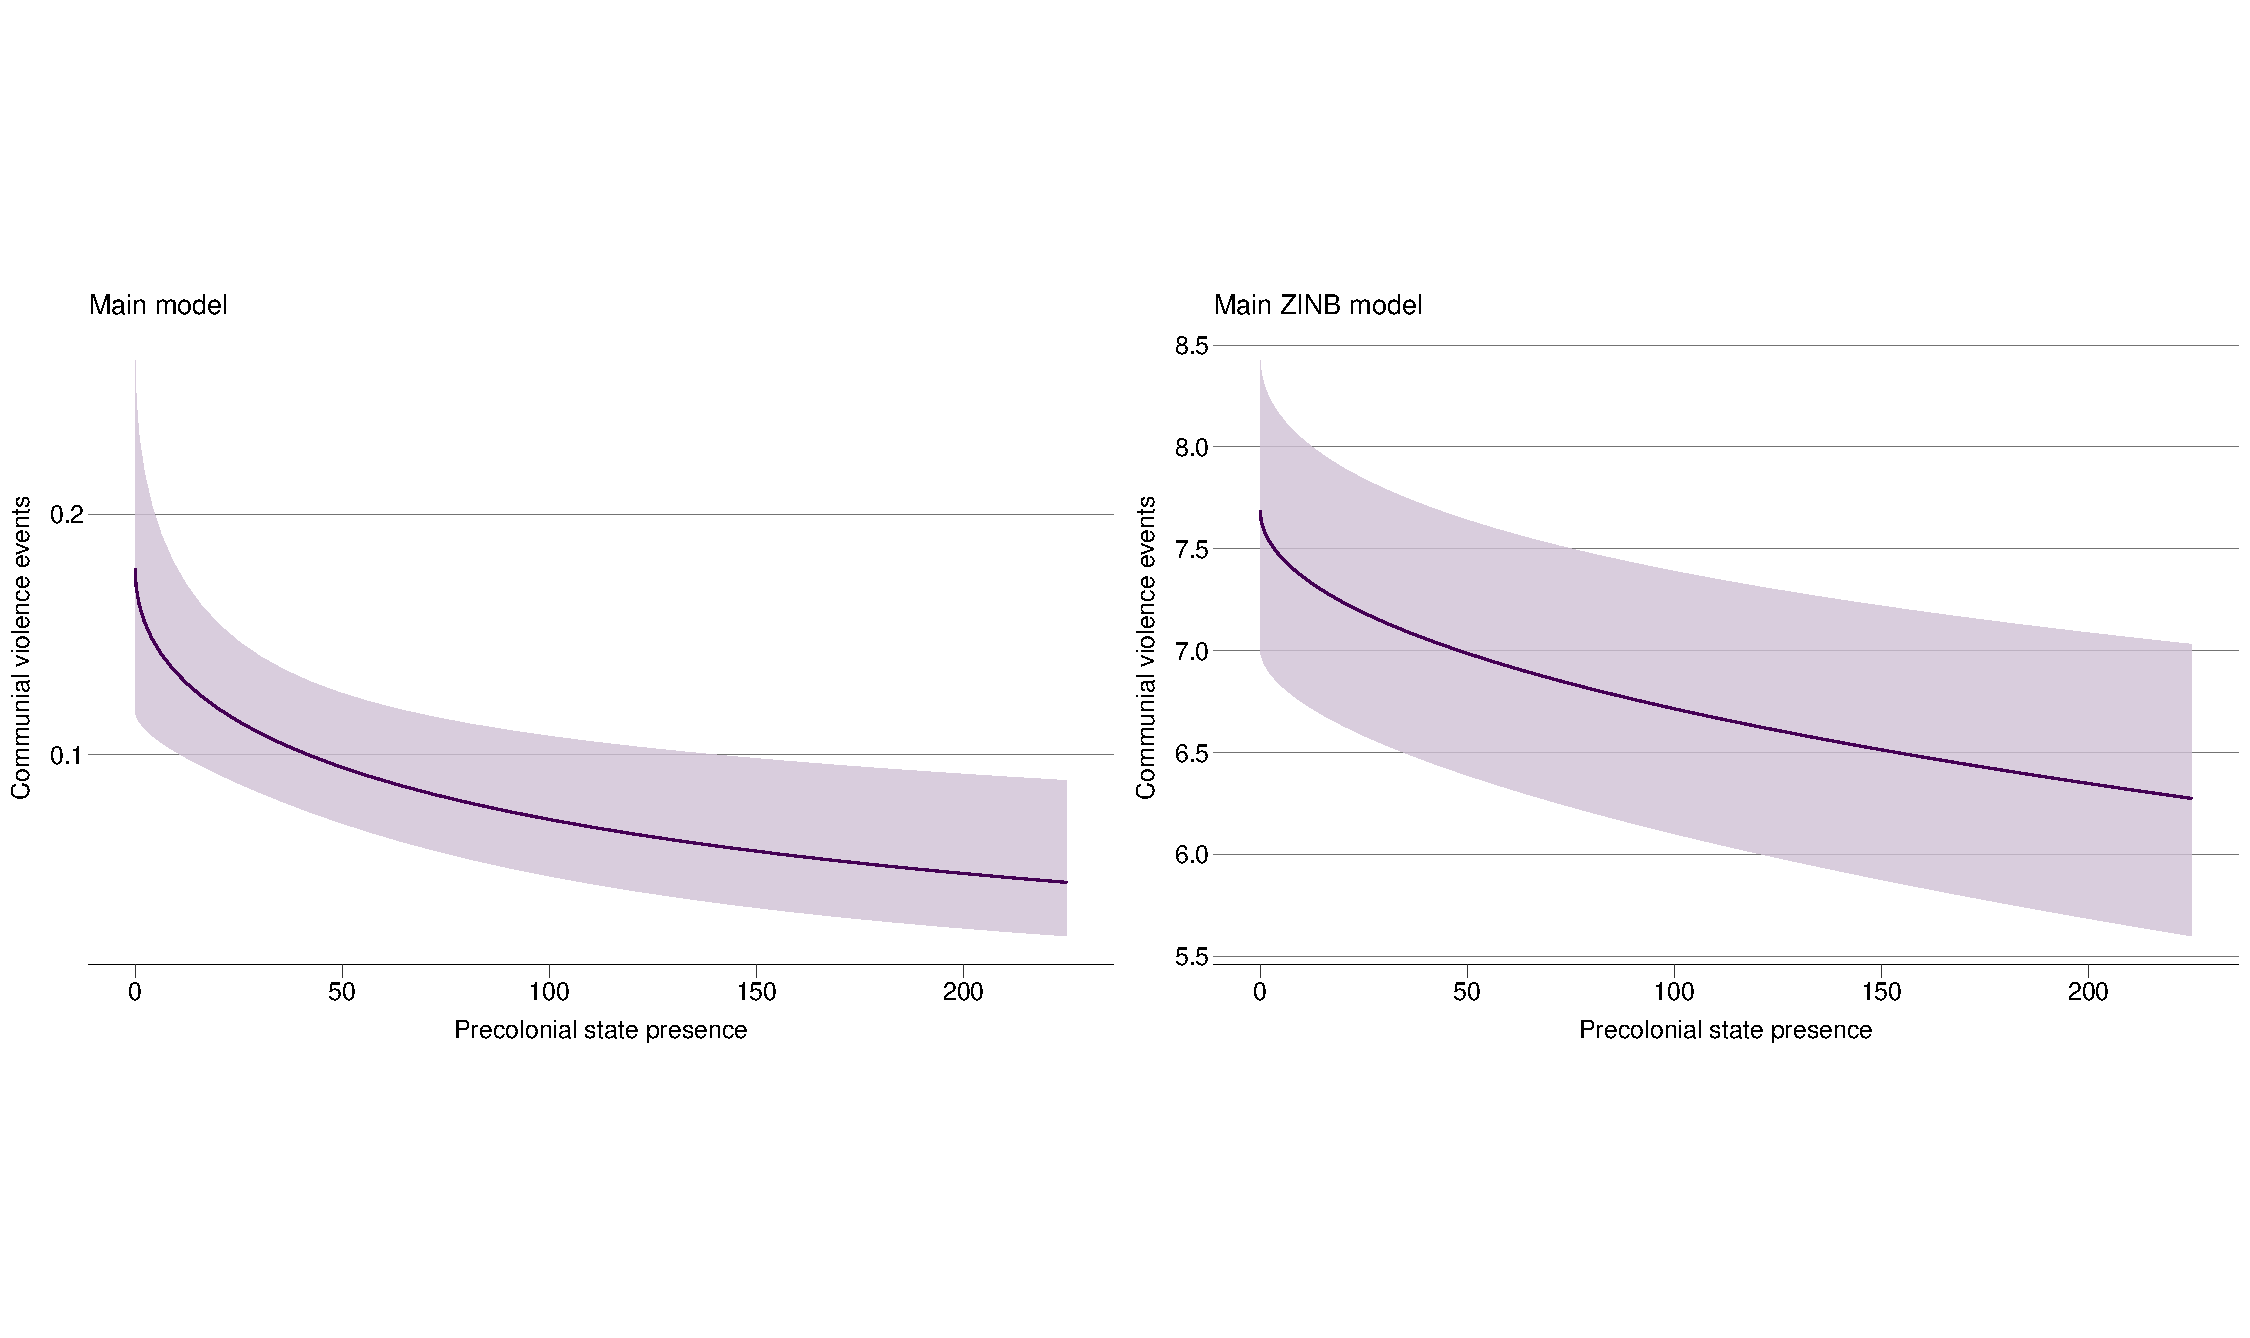
\includegraphics[width=1\linewidth]{R/Output/mainplots.pdf}
	\end{figure}
\end{frame}

\begin{frame}
	\begin{figure}
		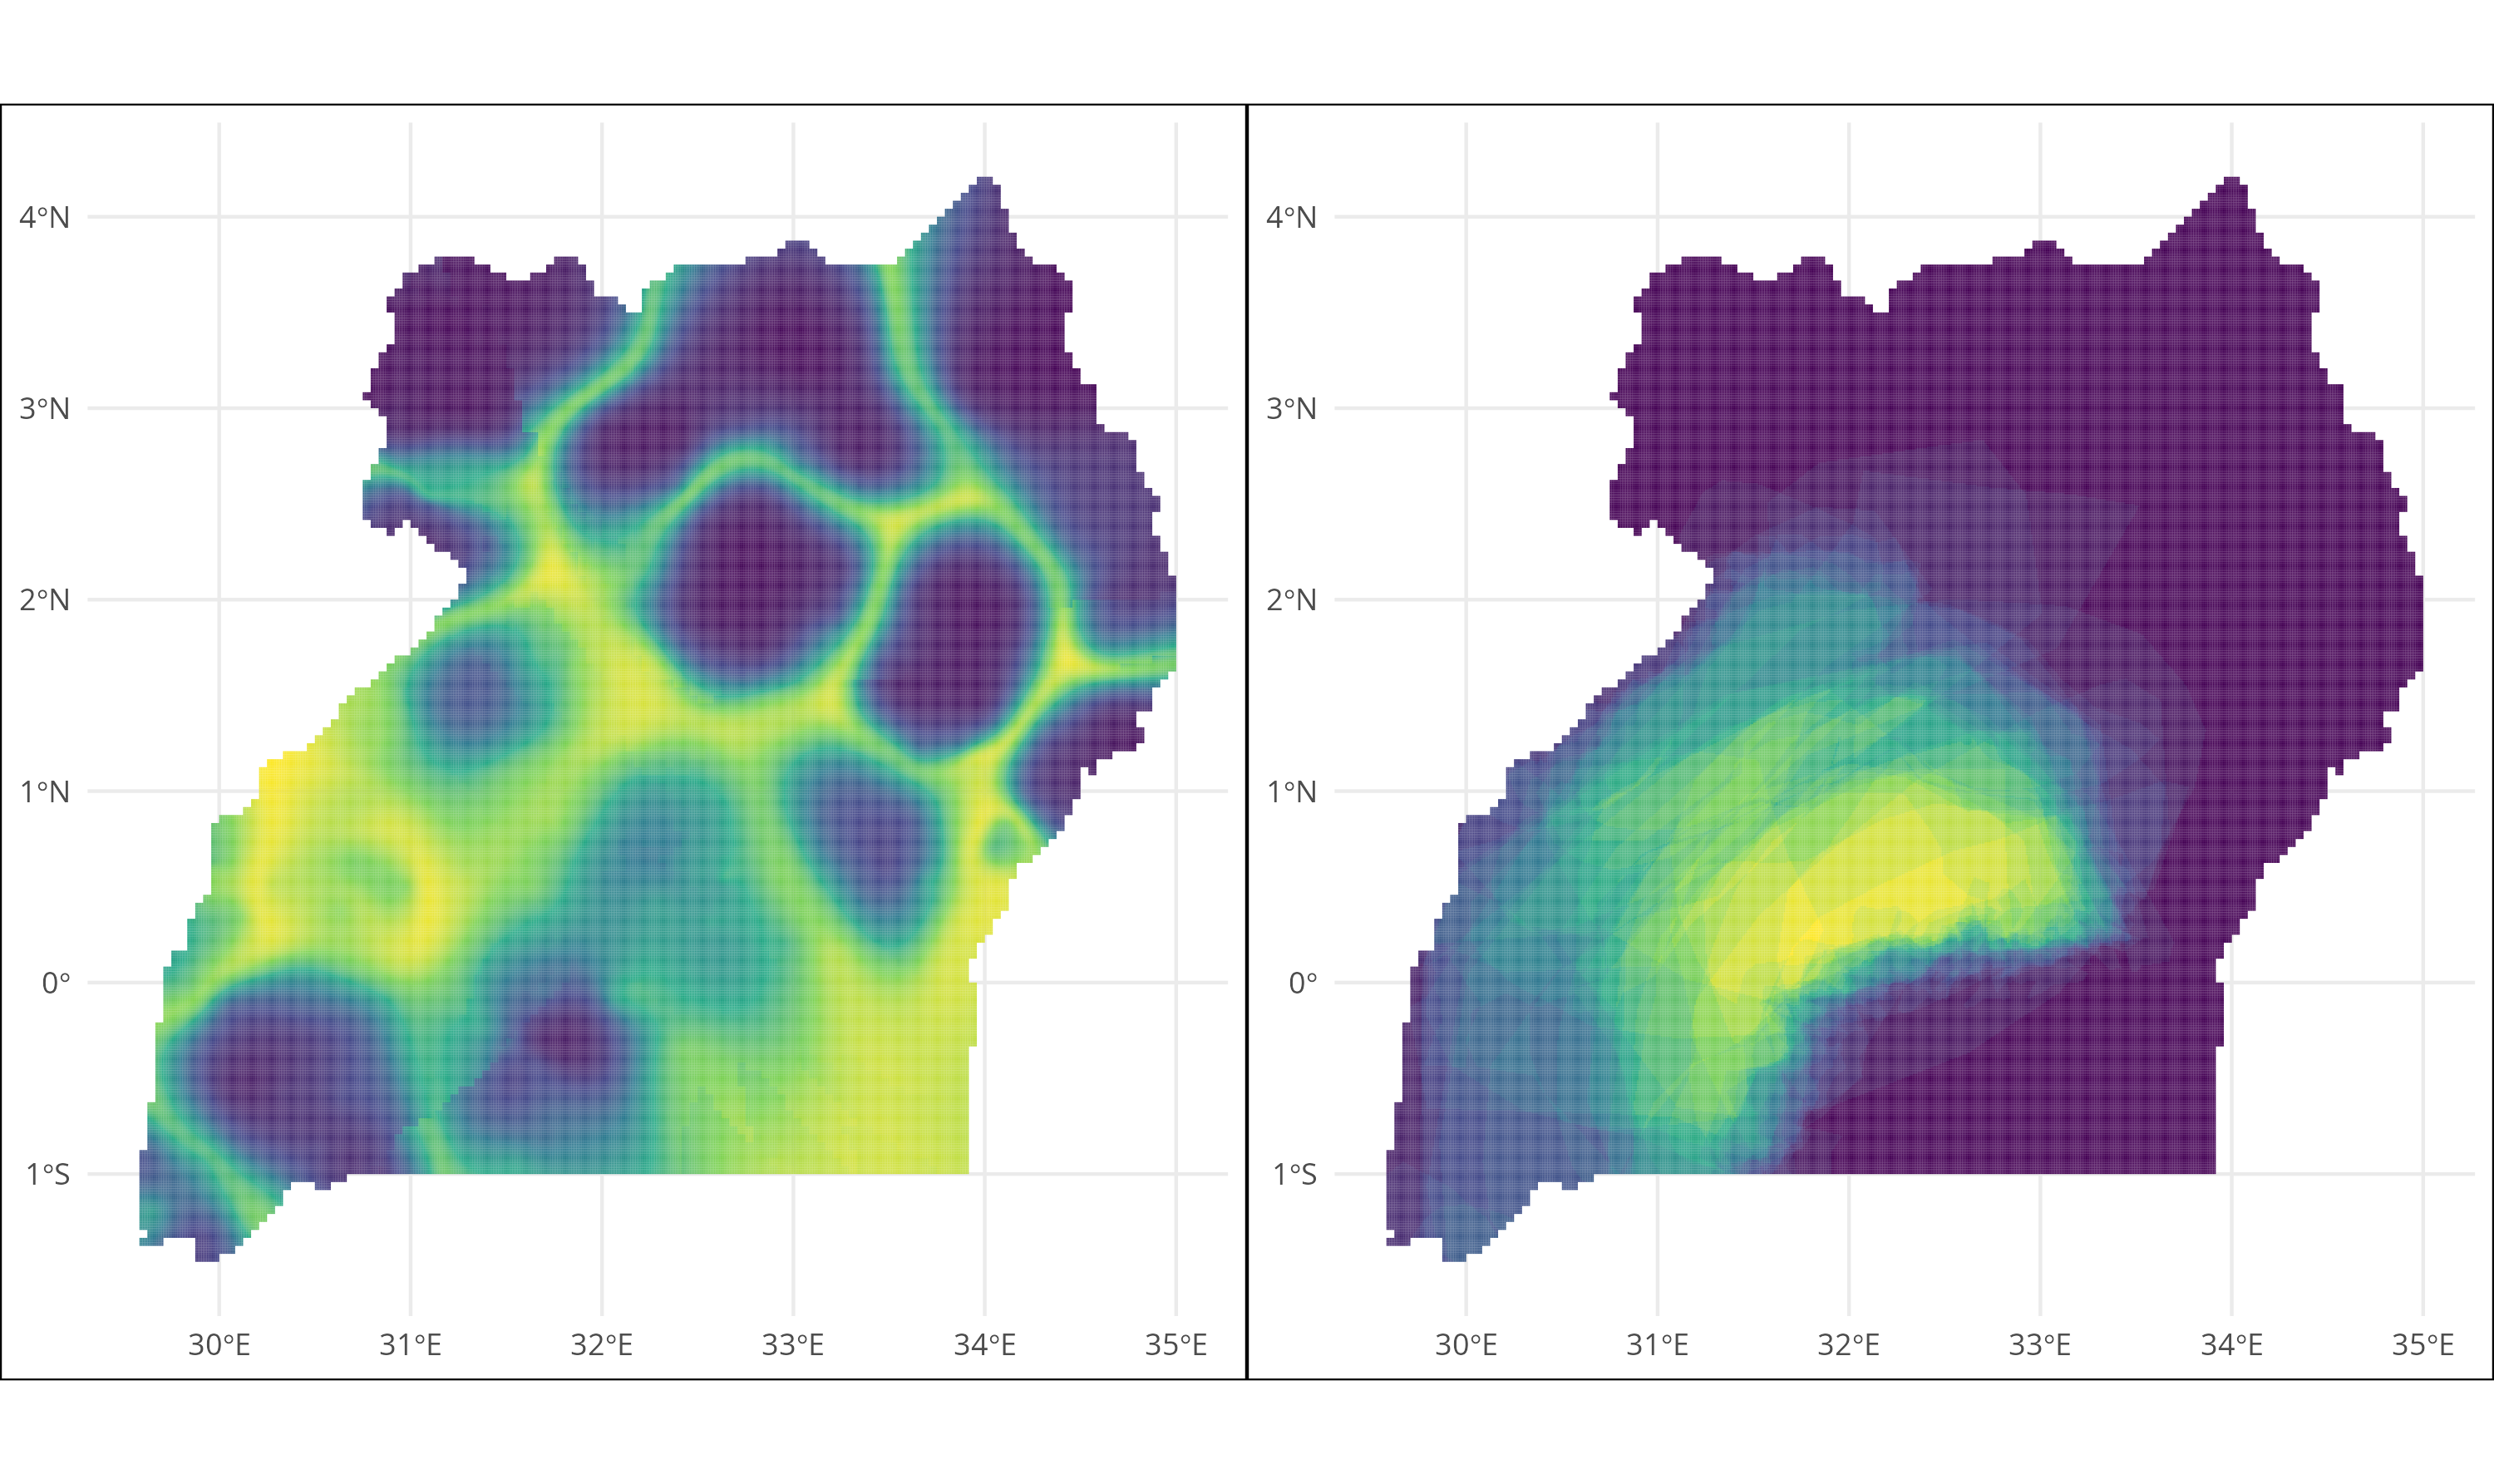
\includegraphics[width=1\linewidth]{img/ugaplots.png}
	\end{figure}
\end{frame}

\end{document}
